\chapter{快照}

\section{概述}

快照,卷是可写快照、当前快照。下文中提及的快照是卷及其快照的统称。

卷是当前快照,可写。卷和快照采用同一元数据结构。

优先选择ROW方案,COW有难以克服的问题。

\hl{从简到繁分阶段实现},设计上要考虑每阶段要解决的主要问题,以及向下一阶段推进的难点所在。
实现按最小功能集的原则进行。最小作用量原理,化整为零。先处理正常流程(normal case),再处理故障情况(exception case)。
\begin{myeasylist}{itemize}
    & normal case
        && non IO
        && IO
    & exception case
        && fail-stop
        && fail-recover
        && mds 切换
\end{myeasylist}

卷的类型
\mygraphics{../imgs/volume-type.png}

\subsection{参与各方}

\mygraphics{../imgs/snapshot/snapshot-component.png}

\hl{没有卷控带来什么影响}?存在卷控的情况下,只需要顺序执行即可。不存在卷控的情况下,转化为了分布式一致性问题。
\begin{myeasylist}{itemize}
    & snapshot structure info
    & read snapshot
\end{myeasylist}

\subsection{各方如何就snaptree达成一致}

\mygraphics{../imgs/snapshot/snapshot-2pc.png}

如何满足事务性是难点。

没有卷控,则创建快照等全局操作可以通过mds master进行。读单个snapshot同读卷。
由mds master维护一个卷的snapshot结构信息。

rangectl必须基于最新snaptree去处理各个操作。\hl{如何让rangectl看见最新snaptree是个难点}。

如何定位snapshot映射到哪个tgtctl上? 不需要!

rangectl控制和数据分离?

每个rangectl都持有最新卷的快照结构信息。

在mds master上,保证同一卷上只有一个快照操作。

在etcd上记录task的状态机,标记其是否完成,重入时,根据该状态机进行必要处理。

unlock之前,必须标记该task已完成。如果放在unlock之后,则如果unlock之后发生故障,重入时会触发undo。
实际上各rangectl上已经unlock,并接受io了。

要保证在任何情况下,系统都是可以满足safety and liveness条件的。

lease = lock + timeout。timeout设为多少合适呢?不如采用undo机制。

广播机制是否可靠?如果有新节点加入会如何?

其它方案:把一个卷的snapshot操作看作io,不用lock?难实施,bactl建立在token连续的假设之下,快照操作并不经过bactl。

\subsection{快照和物理卷的映射关系}

快照和物理卷是1:1的映射关系,一个快照对应一个物理卷。

\subsection{快照如何影响原卷性能}

\section{实现}

\subsection{引入VolumeCtl}

创建、删除等快照操作通过VolumeCtl进行。

\hl{创建和删除快照操作是卷级操作}。如快照树结构发生变化,当如何?
LICH中快照树的变化和访问都是通过卷控做得,所以没有一致性问题。
suzaku中client端充当卷控角色,在多活的情况下,有什么影响?

% 因为快照是只读的,是否可以简化实现?

\subsection{快照树}

一个卷的卷和所有快照构成单根树结构。相关信息持久化到ETCD上。包含指向快照元数据的\hl{chkidx列表}。

% 写IO涉及\hl{当前快照},读IO可能涉及多个快照。
% 快照读与读IO一致,可能涉及多个快照。

% IO的写和读都由client/target进行?在get token里返回物理地址。返回一个或多个token对象?

\subsection{单个快照}

\begin{center}
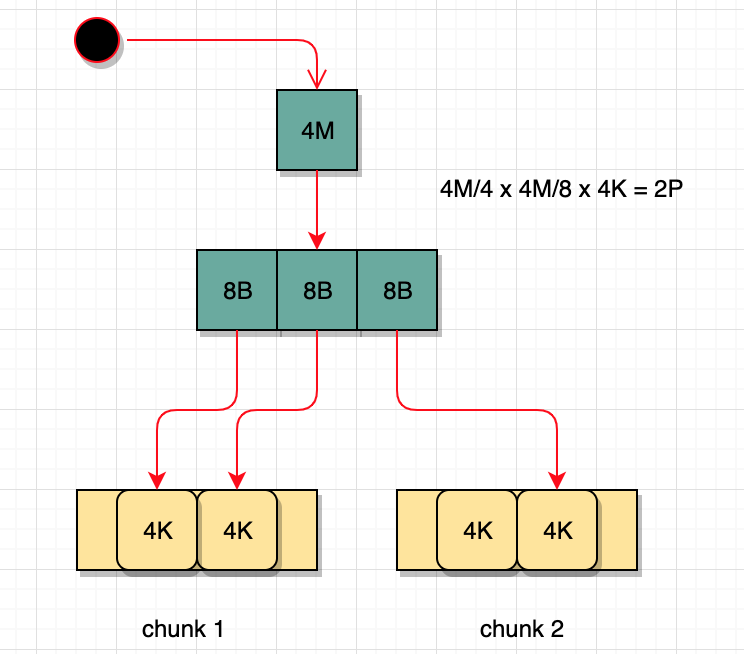
\includegraphics[width=10cm]{../imgs/snapshot/snapshot-head.png}
\end{center}

元数据映射表在哪里维护?与\hl{chunk-副本元数据}一样维护?
% 找get token里返回物理地址。client直接读写该地址。逻辑上连续,物理上未必连续。

% 每个range ctl也维护卷的所有快照的对应范围?按snap name进行索引?
% 当snaptree结构发生变化时,rangectl重新加载?
% 多活的场景下,会有什么问题吗?

如何表示页的物理地址:
\begin{center}
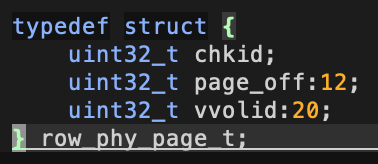
\includegraphics[width=10cm]{../imgs/snapshot/row-phy-page.png}
\end{center}

\subsection{虚拟卷和物理卷的关系}

一种表示法:导出不变的虚拟卷,虚拟卷可以包含多个物理卷,一个快照对应一个物理卷。

另一种表示法:用一个物理卷包含虚拟卷及其快照。

\subsection{Volume Allocator}

封装底层物理卷的访问接口。可以运行在任意backing store上,如file、LUN。

特性:
\begin{enumbox}
\item 引入资源池
\end{enumbox}

优化碎片化的措施:
\begin{enumbox}
\item 事前
\item 事后
\end{enumbox}

\subsection{地址映射}

加入v2p过程:
\begin{center}
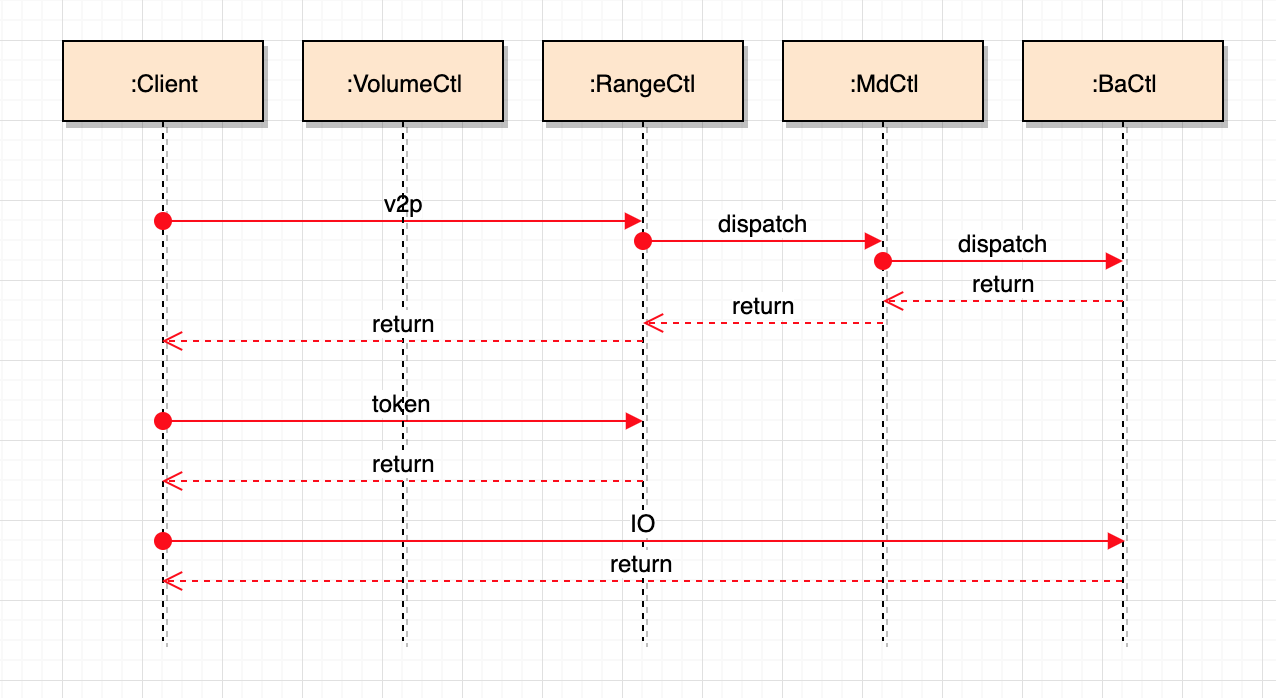
\includegraphics[width=10cm]{../imgs/data-path.png}
\end{center}

\section{TODO}

\begin{myeasylist}{itemize}
    & 限制快照数量
    & 预留空间
    & 超配
    & 调整卷大小
    & 删除卷
    & 快照计划
\end{myeasylist}

\section{参考产品}

\begin{enumbox}
\item SheepDog/SSAN
\item Open VStorage
\item ***
\item FusionSorage
\item NetApp WALFS
\item Dell SC Series
\item 阿里云ECS
\item ***
\item SPDK
\item QEMU qcow2
\end{enumbox}

\subsection{SSAN}

创建snapshot后,快照数据不变,新数据写入卷上,由此可推断SSAN采用了ROW机制,管理粒度是object,不是page-based。

每个快照对应一个快照卷+一个leger卷。leger卷记录对应object的被引用情况。

SSAN的每个卷采用一层元数据,即一个13MB的元数据对象,从而限制了卷的最大大小为4TB。
